\documentclass[aspectratio=169]{beamer}

% PACKAGES
\usepackage{xcolor}
\usepackage{caption}
\usepackage{hyperref}
\hypersetup{
    colorlinks=true,        % false: boxed links; true: colored links.
    allcolors=.,            % So that no previous colors are modified.
    urlcolor=ThemeBlue,     % Color of external links.
    citecolor=ThemeBlue,
}

\usetheme{Patorikku}


\title{Title}
\subtitle{Subtitle}
\author{Authors}
\date{December 18, 2019}
\institute{DSSC - Data Visualisation Exam}


\begin{document}
  % Deactivates slides counter.
  \setcounter{showSlideNumbers}{0}

  % Title page.
  \frame{\titlepage}


  % Initialises and activates slides counter.
  \setcounter{framenumber}{0}
  \setcounter{showSlideNumbers}{1}


  \begin{frame}
    \frametitle{First and last slide}

    Things things things things.

    \vspace{1em} 

    \begin{itemize}
      \item Testo;
      \item Test.
    \end{itemize}

  \end{frame}



  { % all template changes are local to this group.
      \setbeamertemplate{navigation symbols}{}
      \begin{frame}<article:0>[plain]
          \begin{tikzpicture}[remember picture,overlay]
              \node[at=(current page.center)] {
                  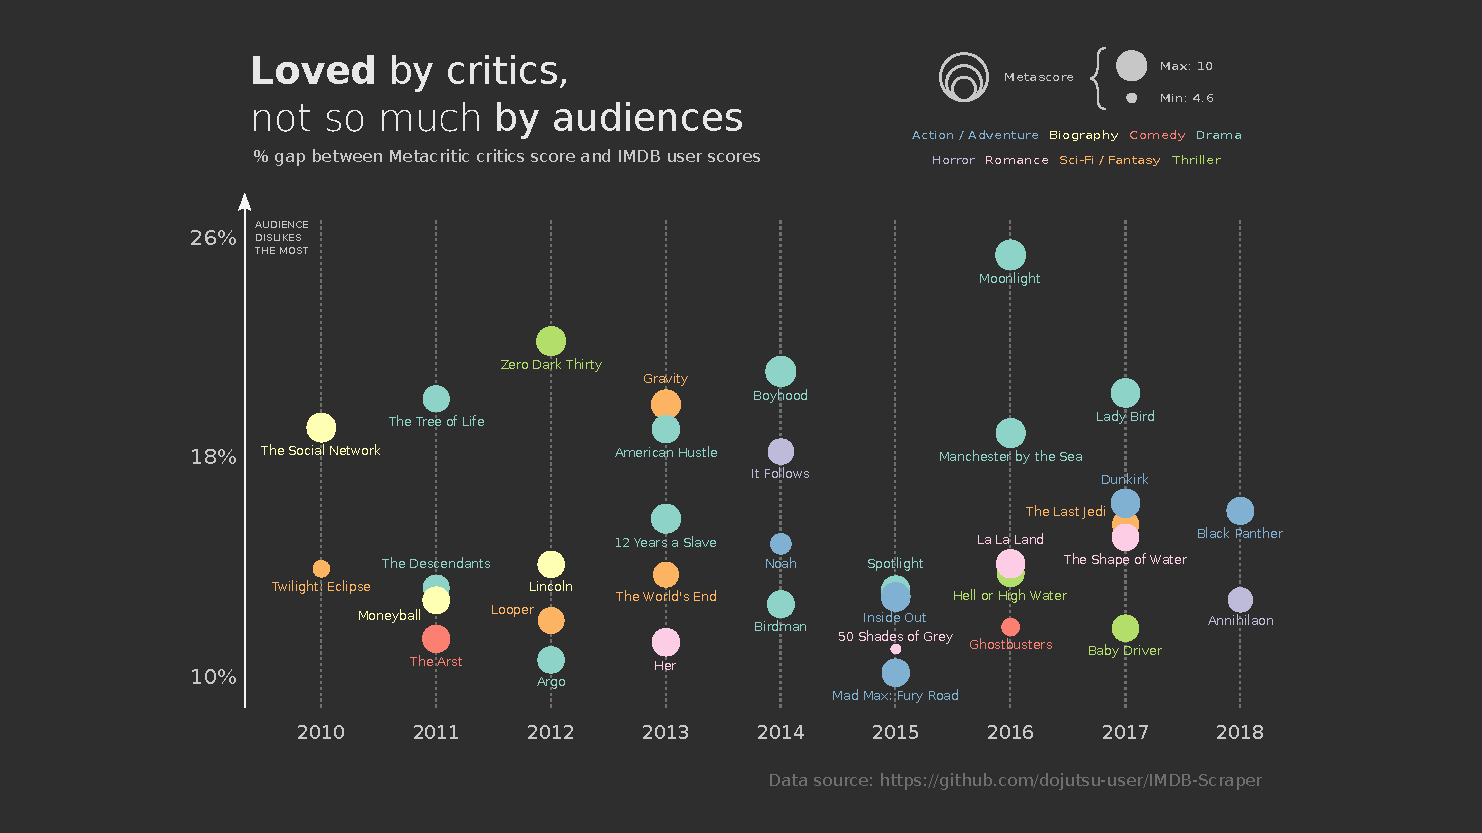
\includegraphics[keepaspectratio,
                                   width=\paperwidth,
                                   height=\paperheight]{img/gap.pdf}
              };
          \end{tikzpicture}
       \end{frame}
  }



  { % all template changes are local to this group.
      \setbeamertemplate{navigation symbols}{}
      \begin{frame}<article:0>[plain]
          \begin{tikzpicture}[remember picture,overlay]
              \node[at=(current page.center)] {
                  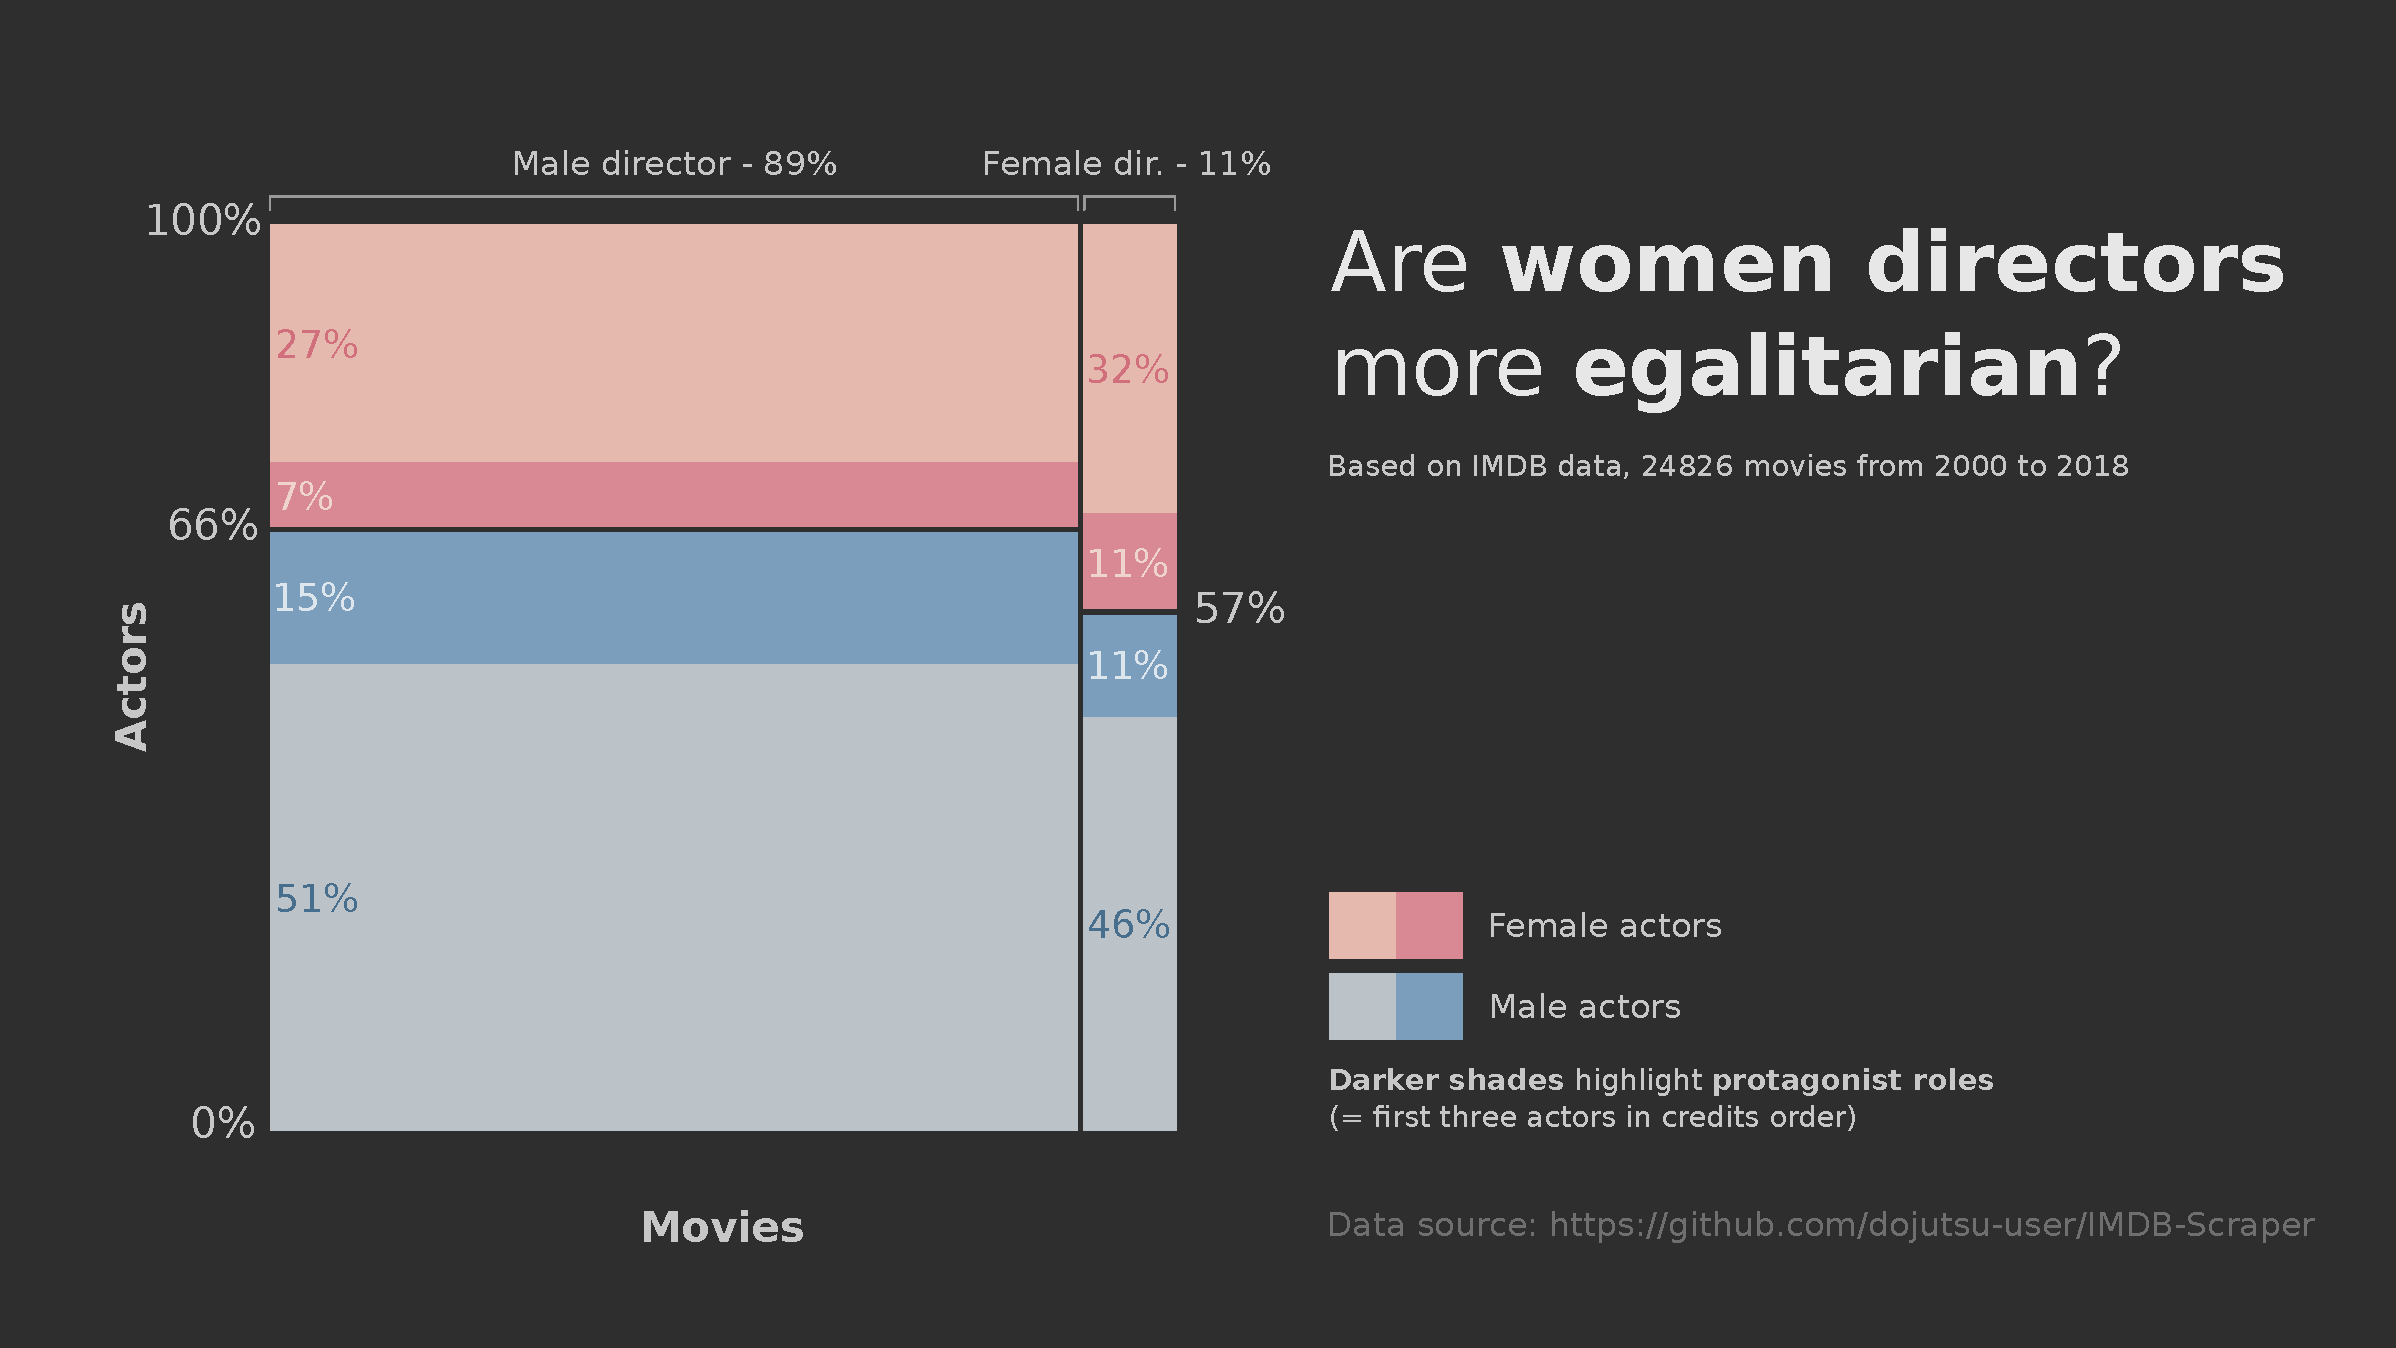
\includegraphics[keepaspectratio,
                                   width=\paperwidth,
                                   height=\paperheight]{img/gender_v2.pdf}
              };
          \end{tikzpicture}
       \end{frame}
  }


  { % all template changes are local to this group.
      \setbeamertemplate{navigation symbols}{}
      \begin{frame}<article:0>[plain]
          \begin{tikzpicture}[remember picture,overlay]
              \node[at=(current page.center)] {
                  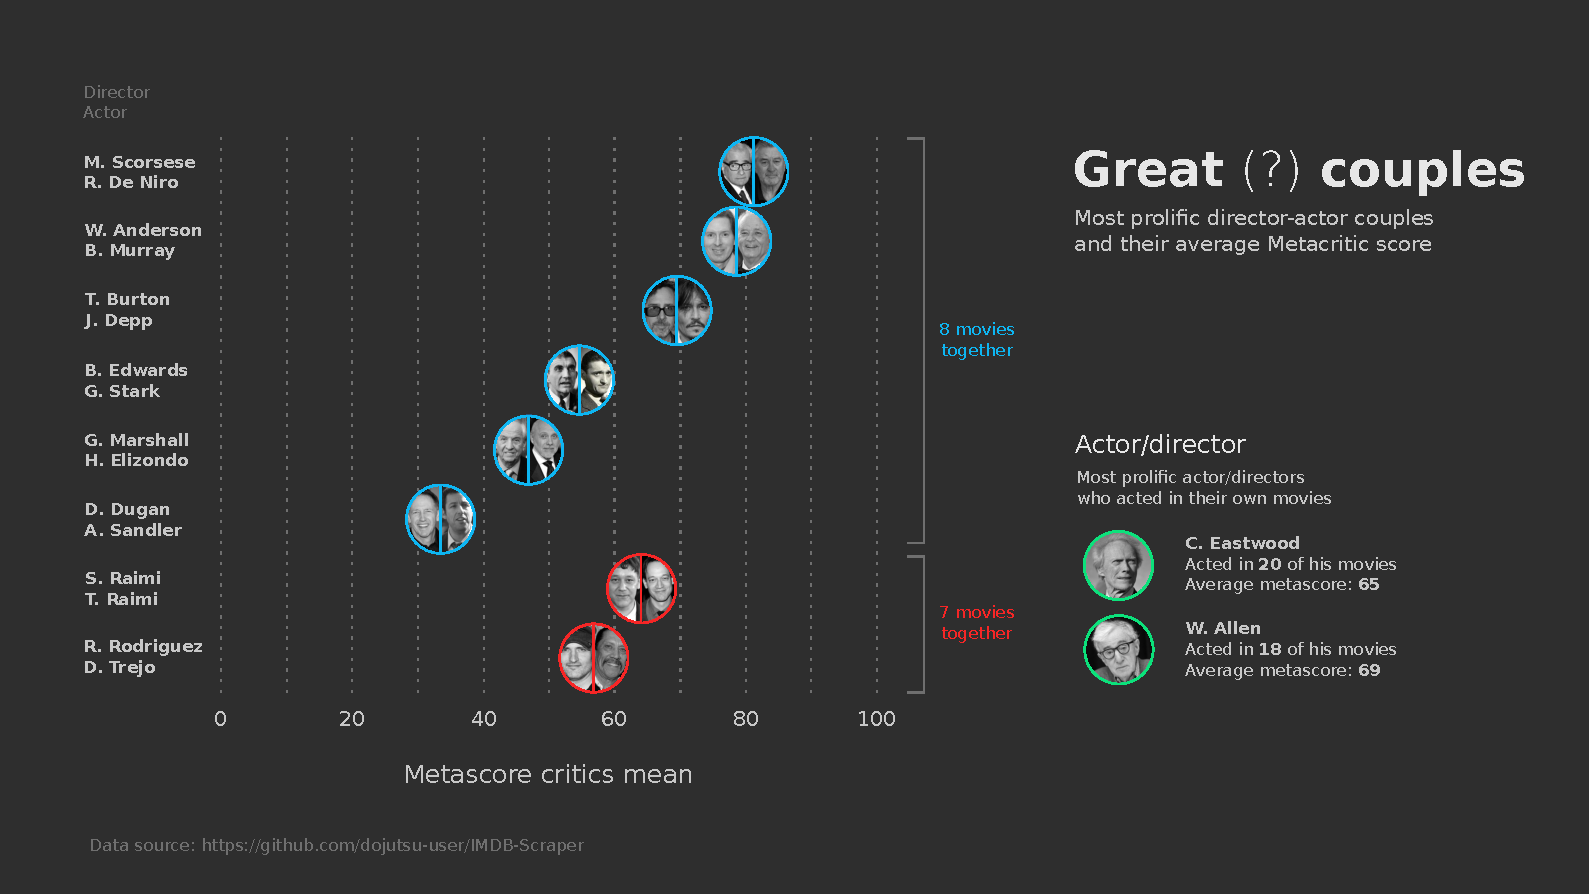
\includegraphics[keepaspectratio,
                                   width=\paperwidth,
                                   height=\paperheight]{img/couples.pdf}
              };
          \end{tikzpicture}
       \end{frame}
  }



  \begin{frame}
    \frametitle{References}

    \nocite{*}

    \setbeamercolor{bibliography entry author}{fg=ThemeRed}
    \setbeamercolor{bibliography entry title}{fg=black} 
    \setbeamercolor{bibliography entry location}{fg=black} 
    \setbeamercolor{bibliography entry note}{fg=black}  
    \setbeamercolor{bibliography item}{fg=ThemeBlue}
    \setbeamertemplate{bibliography item}[text]

    \bibliographystyle{abbrv}
    \footnotesize{
      \bibliography{biblio.bib} 
    }
  \end{frame}



\end{document}
